\section{ГЛАВА 4 ПРОЕКТИРОВАНИЕ АРХИТЕКТУРЫ И ВЫБОР ТЕХНОЛОГИЧЕСКОГО СТЕКА}

\subsection*{Введение}

В предыдущей главе были определены ключевые функциональные требования и приоритеты для мобильного приложения, направленного на удовлетворение потребностей различных групп пользователей в сфере туризма и путешествий. Для успешной реализации задуманного продукта необходимо тщательно продумать архитектуру приложения и механизмы взаимодействия между его компонентами.

Данная глава посвящена детальному проектированию технической инфраструктуры приложения, включая архитектуру мобильного клиента и API для взаимодействия с бэкендом. Проработка этих аспектов позволит обеспечить эффективное функционирование приложения, его масштабируемость и возможность интеграции с внешними системами.

Основные задачи, решаемые в ходе работы:

% \begin{enumerate}
%     \item Проектирование архитектуры приложения с упором на принципы SOLID \footnote{SOLID – акроним для пяти принципов объектно-ориентированного проектирования: Single Responsibility Principle (Принцип единственной ответственности), Open/Closed Principle (Принцип открытости/закрытости), Liskov Substitution Principle (Принцип подстановки Барбары Лисков), Interface Segregation Principle (Принцип разделения интерфейса) и Dependency Inversion Principle (Принцип инверсии зависимостей)}. Например, KISS\footnote{KISS (Keep It Simple, Stupid) – принцип проектирования, который призывает к простоте и отказу от излишней сложности в системе.} и DRY\footnote{DRY (Don\'t Repeat Yourself) – принцип разработки программного обеспечения, направленный на снижение повторения информации различного рода, особенно в системах со множеством слоев абстрагирования.}.
%     \item Разработка пользовательского интерфейса (UI\footnote{UI (User Interface) – пользовательский интерфейс, совокупность средств, при помощи которых пользователь взаимодействует с различными устройствами, программами и веб-сайтами. В Flutter UI строится с помощью виджетов.)} с учетом современных практик UX \footnote{UX (User Experience) – пользовательский опыт, совокупность впечатлений и эмоций, которые испытывает пользователь при взаимодействии с продуктом, системой или услугой.}.
% \end{enumerate}

\subsection*{Цели и задачи главы}

\begin{itemize}
    \item Проектирование архитектуры мобильного приложения с упором на принципы SOLID \footnote{SOLID – акроним для пяти принципов объектно-ориентированного проектирования: Single Responsibility Principle (Принцип единственной ответственности), Open/Closed Principle (Принцип открытости/закрытости), Liskov Substitution Principle (Принцип подстановки Барбары Лисков), Interface Segregation Principle (Принцип разделения интерфейса) и Dependency Inversion Principle (Принцип инверсии зависимостей)}. Например, KISS\footnote{KISS (Keep It Simple, Stupid) – принцип проектирования, который призывает к простоте и отказу от излишней сложности в системе.} и DRY\footnote{DRY (Don\'t Repeat Yourself) – принцип разработки программного обеспечения, направленный на снижение повторения информации различного рода, особенно в системах со множеством слоев абстрагирования.}.
    \item Разработка спецификации API для взаимодействия мобильного клиента с бэкенд-сервисами, обеспечивающие обмен необходимыми данными и функциональностью.
    \item Выявление потенциальные сложности и предложить пути их решения на этапе проектирования архитектуры и API.
\end{itemize}

\subsection*{Структура главы}

\begin{itemize}
    \item \textbf{4.1. Проектирование архитектуры мобильного приложения} — в этом разделе будет рассмотрена выбор технологической стопки, структура приложения, подходы к организации кода и данные, необходимые для корректной работы приложения.
    \item \textbf{4.2. Проработка API для взаимодействия с бэкендом} — здесь будут описаны требования к API, структура запросов и ответов, механизмы аутентификации и авторизации, а также примеры использования API для основных сценариев взаимодействия между клиентом и сервером.
\end{itemize}

\subsection*{4.1 Проектирование архитектуры мобильного приложения}
\addcontentsline{toc}{subsection}{4.1 Проектирование архитектуры мобильного приложения}


\subsubsection*{Технические требования (SRS)}


Для проектирования эффективной архитектуры необходимо четко понимать задачи, которые должно решать приложение, и как пользователи будут с ним взаимодействовать. В процессе разработки мобильного приложения для сферы туризма и путешествий особое внимание уделяется техническим аспектам, которые обеспечивают его функциональность, удобство использования и безопасность. Технические требования (SRS) играют ключевую роль в определении основных характеристик приложения и его взаимодействия с пользователем и внешними системами.

На данном этапе разработки важно детально проработать технические аспекты, чтобы обеспечить соответствие приложения ожиданиям пользователей и требованиям рынка. Это включает в себя выбор платформы, разработку пользовательского интерфейса, обеспечение безопасности данных и интеграцию с внешними сервисами.

На основе анализа, проведенного в Главе 1 и общих целей проекта, были сформулированы следующие ключевые аспекты следующие технические требования:


\begin{itemize}
    \item \textbf{Поддержка iOS и Android}: приложение должно быть доступно для пользователей устройств на базе операционных систем iOS и Android. Это обеспечит широкий охват аудитории и возможность использования приложения на различных устройствах. Разработка под обе платформы позволяет охватить максимальное количество потенциальных пользователей и обеспечивает гибкость в выборе устройства для доступа к приложению. Выбор кроссплатформенного фреймворка Flutter позволяет поддерживать обе эти платформы из коробки с наименьшей затратой усилий по сравнению с нативной разработкой под каждую из этих платформ.
    \item \textbf{Интуитивная понятность}: интерфейс приложения должен быть разработан таким образом, чтобы пользователи могли легко ориентироваться и выполнять необходимые действия без дополнительных инструкций. Это достигается за счёт логичной структуры меню, понятных иконок и чётких инструкций.
    \item \textbf{Адаптивность}: дизайн интерфейса должен быть адаптирован под различные размеры экранов мобильных устройств, обеспечивая оптимальное отображение и удобство использования. Адаптивный дизайн позволяет приложению корректно отображаться на смартфонах и планшетах с разными диагоналями экранов.
    \item \textbf{Визуальная привлекательность}: интерфейс должен иметь привлекательный и современный дизайн, который будет соответствовать ожиданиям пользователей и способствовать положительному восприятию приложения. Визуальная составляющая играет важную роль в создании первого впечатления и удержании интереса пользователей.
    \item \textbf{Защита персональных данных}: приложение должно обеспечивать надёжную защиту персональных данных пользователей, включая их имена, адреса, номера телефонов и другую конфиденциальную информацию. Это достигается путём использования современных криптографических методов и соблюдения требований законодательства в области защиты данных. Защита данных повышает доверие пользователей к приложению и соответствует юридическим нормам.
    \item \textbf{Аутентификация и авторизация}: реализация механизмов аутентификации и авторизации пользователей для обеспечения доступа к персональным данным и функциональности приложения только для авторизованных пользователей. Это предотвращает несанкционированный доступ к чувствительной информации и обеспечивает безопасность пользовательских данных.
    \item \textbf{Внешние сервисы}: приложение должно предоставлять возможность интеграции с картографическими сервисами, такими как Яндекс Карты и 2GIS, для просмотра маршрутов. Это позволит пользователям получать дополнительные данные о местах, строить маршруты и просматривать информацию о достопримечательностях прямо из приложения. Интеграция с внешними сервисами расширяет функциональность приложения и улучшает пользовательский опыт. Для безопасного открытия этих приложений, можно завести диплинки \footnote[0]{\textbf{диплинк} - гиперссылка, которая открывает конкретную страницу в приложении}.
\end{itemize}

\noindent Первые три пункта помогают снизить количество ошибок в продакшене и сделать их более предсказуемыми. Последний пункт важен для обеспечения отзывчивости пользовательского интерфейса, так как долгие операции не должны блокировать основной поток выполнения, ответственный за отрисовку интерфейса.

\subsection*{4.2 Основные пути пользователя}
\addcontentsline{toc}{subsection}{4.2 Основные пути пользователя}

Путь пользователя (user journey) - это последовательность шагов, которую предпринимает пользователь для того, чтобы завершить конкретную задачу на сайте или в приложении. Для реализации максимально удобного функционала необходимо понимать самые частые пути пользователя и делать их наиболее простыми для него.

В нашем приложении можно выделить следующие основные пути пользователя:

\begin{itemize}
    \item \textbf{Поиск маршрута} - это главная цель  пользователя, найти тот самый маршрут, который он захочет пройти. Эта функция позволяет пользователям быстро и удобно находить маршруты, соответствующие их интересам и потребностям. Они могут использовать различные критерии для поиска, такие как местоположение, тип маршрута, длина и сложность. После выбора маршрута пользователи могут просмотреть его детали, включая карту, описание и фотографии, чтобы лучше понять, что их ждёт во время путешествия. Посмотреть путь, который придётся пройти пользователю, чтобы найти маршрут, можно увидеть на рисунке 2.1.
    \begin{figure}[H]
        \centering
        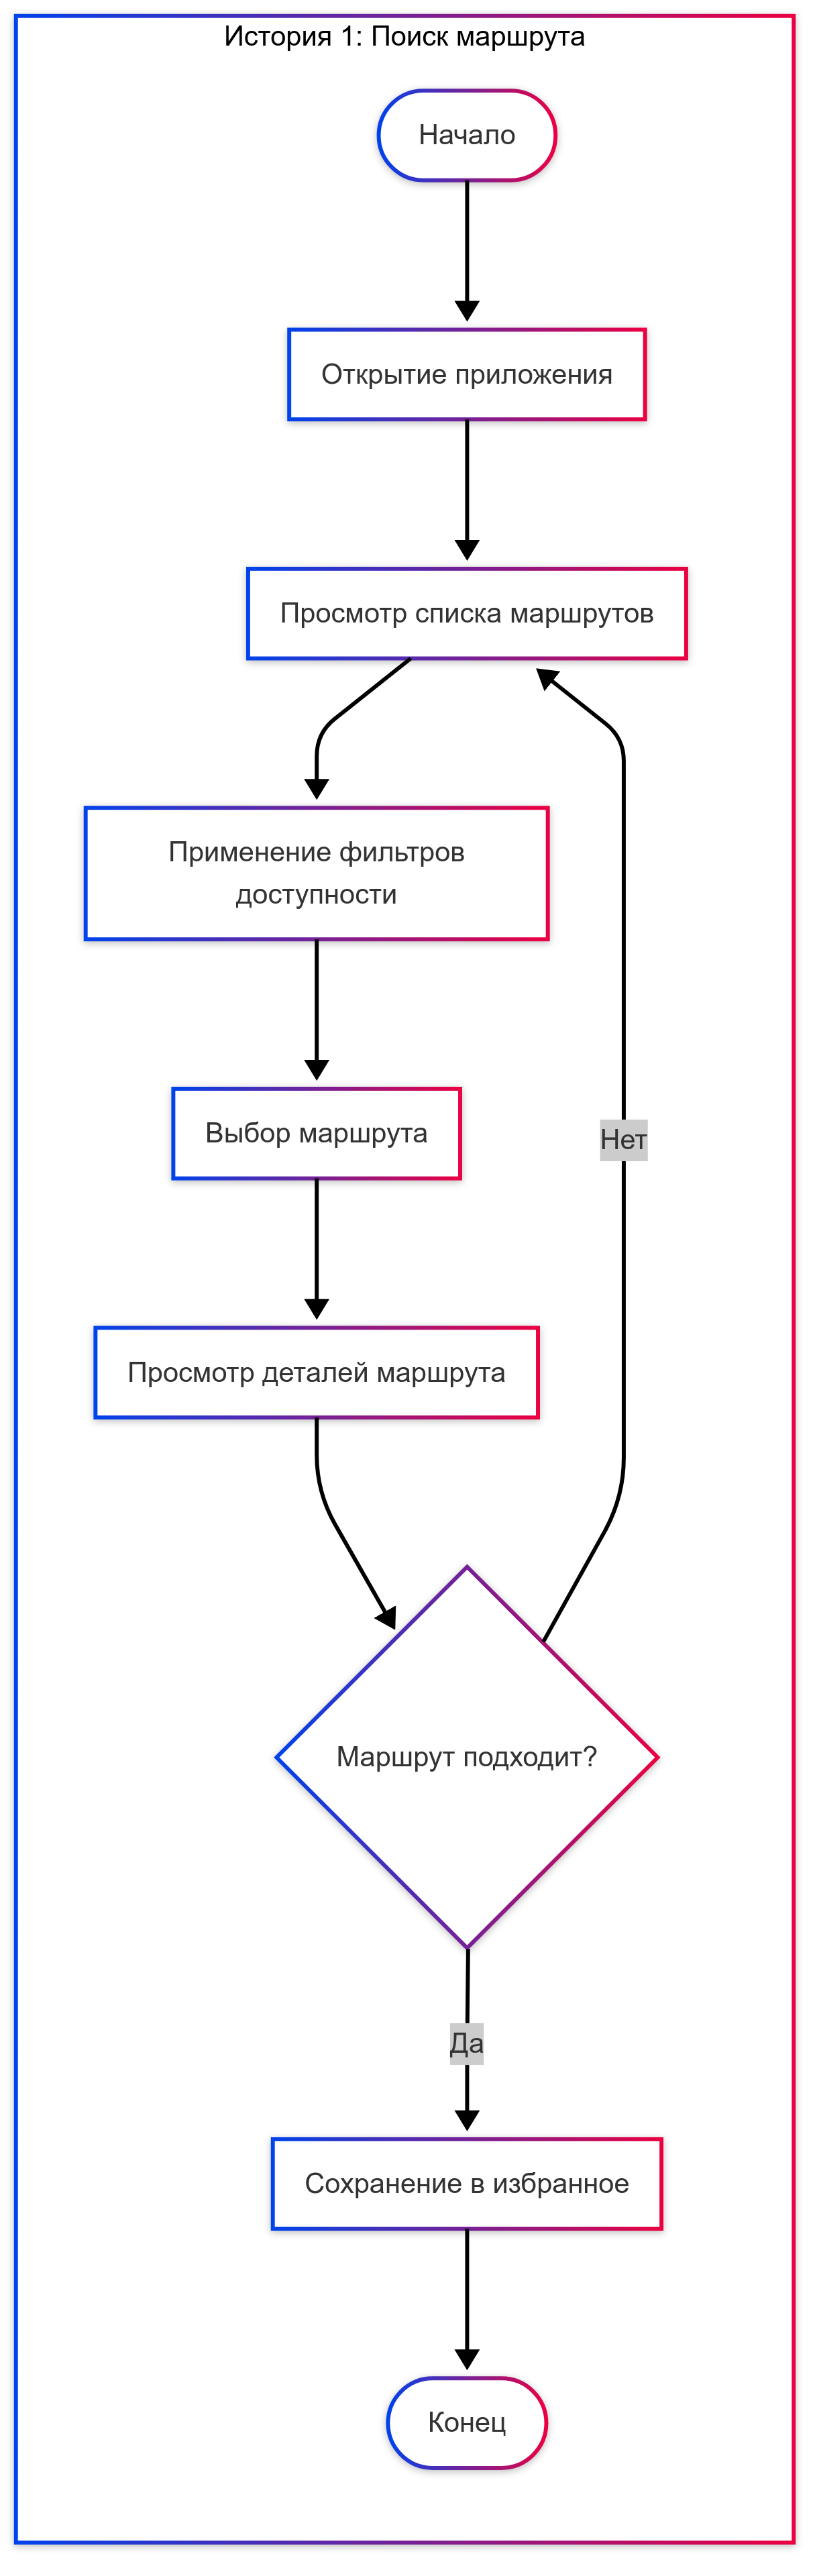
\includegraphics[width=0.4\linewidth]{Images/mobile_logic/история_поиск_маршрута-2025-04-13-175239.png}
        \caption{Диаграмма «Поиск маршрута»}
        \label{fig:enter-label}
    \end{figure}
    \item \textbf{Создание маршрута} - создание маршрута также важная часть функционала, которая позволяет пользователям делиться своими любимыми маршрутами с другими. Пользователи могут создавать маршруты, добавляя точки интереса, описания и фотографии. Это даёт возможность не только планировать свои путешествия, но и помогать другим пользователям находить интересные места и маршруты. Чтобы узнать, что должен сделать пользователь, чтобы создать маршрут, нужно открыть рисунок 2.2.
    \begin{figure}
        \centering
        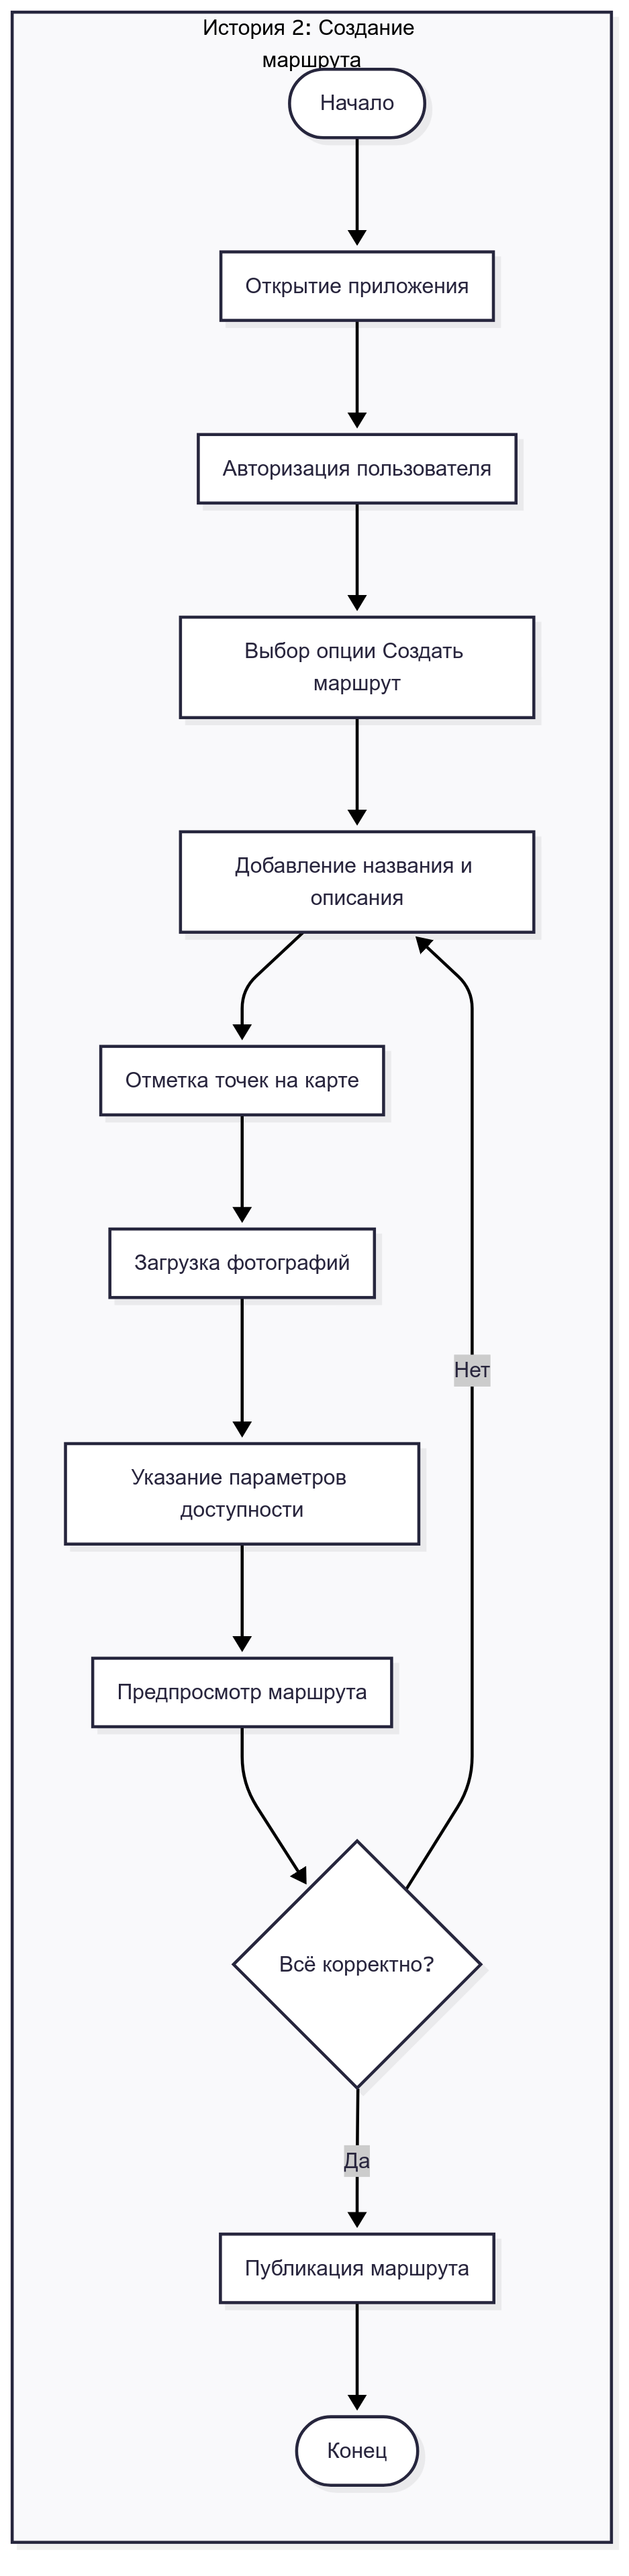
\includegraphics[width=0.3\linewidth]{Images/mobile_logic/создание_маршрута-2025-04-13-180512.png}
        \caption{Диаграмма «Создание маршрута»}
        \label{fig:enter-label}
    \end{figure}
\end{itemize}

\subsubsection*{Диаграмма вариантов использования}

Как было замечено ранее, у нашего приложения будут два основных пользователя: создатель и потребитель маршрута. Диаграмма вариантов использования является важным инструментом для визуализации взаимодействия между пользователями и системой. В контексте нашего приложения можно выделить два основных типа пользователей: создатель маршрута и потребитель маршрута. Наш сервис выступает в роли посредника, обеспечивая взаимодействие между этими двумя сторонами.

\textbf{Создатель маршрута} — это пользователь, который создаёт новые маршруты, добавляя в них информацию о точках интереса, описания, фотографии и другие данные. Он использует наш сервис для публикации маршрутов, которые затем могут быть найдены и использованы другими пользователями — потребителями маршрутов.

\textbf{Потребитель маршрута} — это пользователь, который ищет интересные маршруты для своих путешествий. Он использует наш сервис для поиска, просмотра и сохранения маршрутов, созданных другими пользователями. Потребитель может оценивать маршруты, оставлять комментарии и делиться ими с друзьями.

Наш сервис предоставляет функциональность, необходимую для создания, управления и просмотра маршрутов. Он обеспечивает безопасное и удобное взаимодействие между создателями и потребителями маршрутов, а также предоставляет дополнительные возможности, такие как фильтрация маршрутов по различным критериям, сохранение маршрутов в избранное и получение уведомлений о новых маршрутах.

Так как наш сервис будет проводником между этими двумя сторонами, в следующей диаграмме вариантов использования фигурируют три стороны: наш сервис, создатель и потребитель маршрута. Как именно они связаны, можно увидеть на рисунке 2.3.

Диаграмма вариантов использования демонстрирует следующие взаимодействия:

\begin{enumerate}
    \item \textbf{Просмотр маршрутов}: потребитель маршрутов взаимодействует с нашим сервисом для просмотра списка доступных маршрутов.
    \item \textbf{Редактирование маршрута}: потребитель может редактировать маршрут, и наш сервис отображает отредактированный маршрут.
    \item \textbf{Фильтрация маршрутов}: потребитель использует функционал фильтрации для поиска маршрутов по определённым критериям, и сервис отображает отфильтрованные маршруты.
    \item \textbf{Сохранение маршрута в избранное}: потребитель может сохранять маршруты в избранное, и сервис подтверждает сохранение.
    \item \textbf{Комментирование маршрута}: потребитель может оставлять комментарии к маршрутам, и сервис отображает комментарии.
    \item \textbf{Создание нового маршрута}: создатель маршрута взаимодействует с сервисом для создания нового маршрута, и сервис подтверждает создание.
    \item \textbf{Редактирование маршрута}: создатель может редактировать маршрут, и сервис отображает отредактированный маршрут.
\end{enumerate}

\begin{figure}[h!]
    \centering
    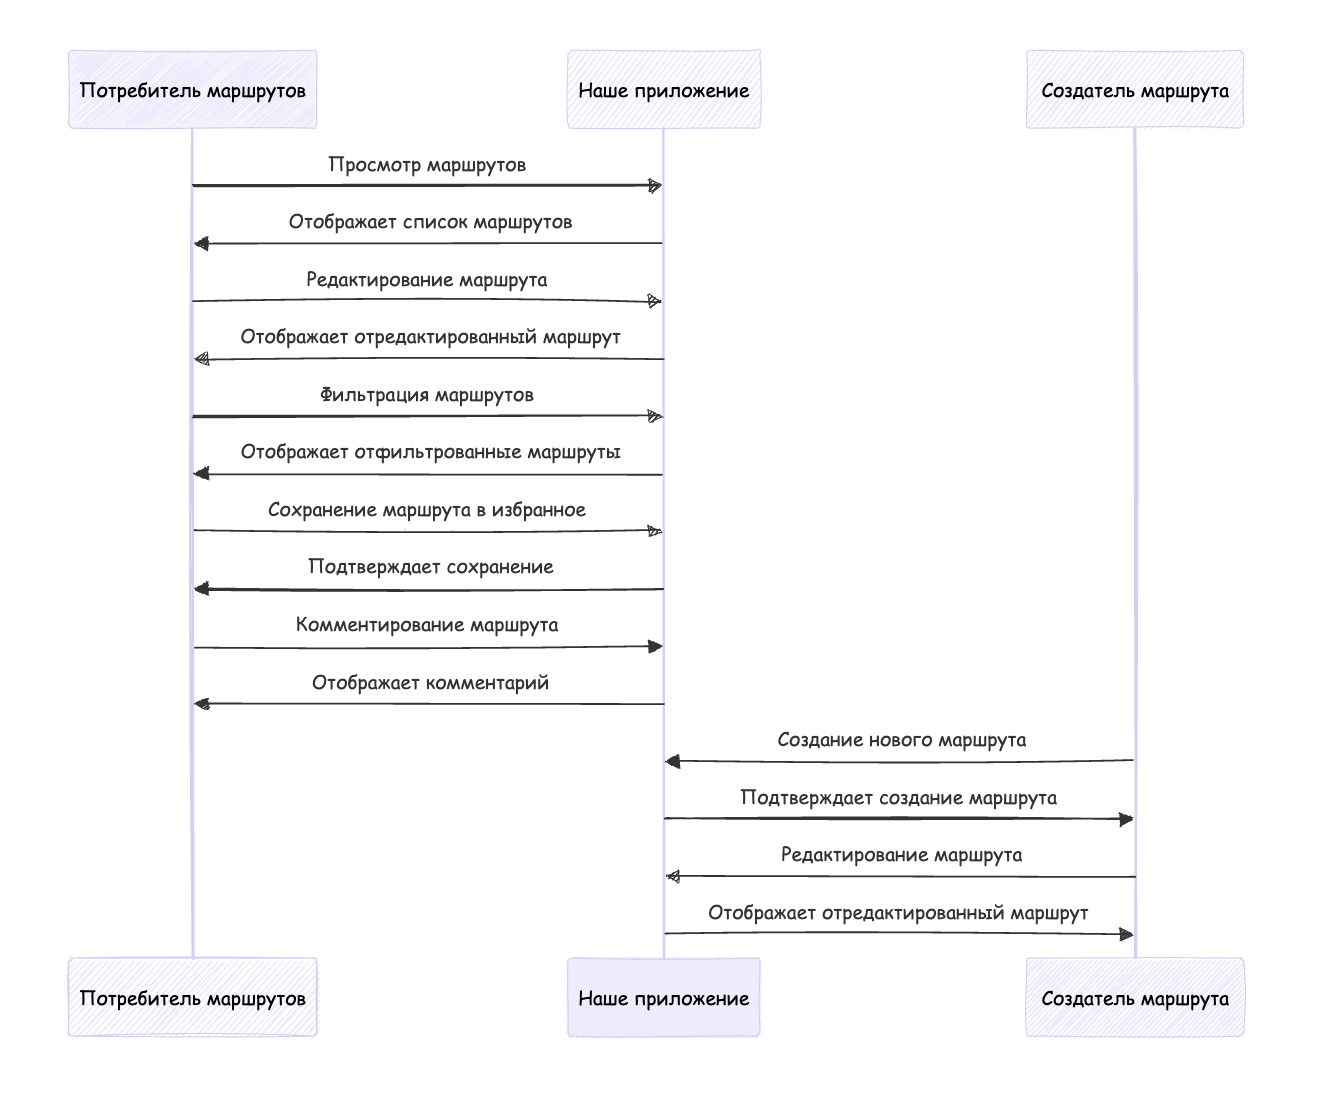
\includegraphics[width=1\linewidth]{Images/mobile_logic/диаграмма_вариантов_использования.png}
    \caption{Диаграмма вариантов использования приложения}
    \label{fig:enter-label}
\end{figure}

\subsection*{4.3 Архитектура мобильного приложения}
\addcontentsline{toc}{subsection}{4.3 Архитектура мобильного приложения}


После проработки требований и сценариев можно приступить к выбору архитектуры мобильного приложения. Но перед этим необходимо дать определение термину архитектура. 

Выбор архитектуры является критически важным решением, влияющим на все аспекты жизненного цикла программного продукта. \textbf{Архитектура программного обеспечения} — это фундаментальная организация системы, воплощенная в ее компонентах, их взаимоотношениях друг с другом и окружением, а также принципы, направляющие ее проектирование и эволюцию.


При разработке мобильного приложения для путешествий на Flutter одним из ключевых решений является выбор архитектуры. Архитектура определяет структуру приложения, распределение ответственности между компонентами и влияет на такие аспекты, как масштабируемость, тестируемость и сопровождаемость кода. Для начала важно выбрать архитектуру для управления состоянием приложения, для этого рассмотрим основные архитектуры, применяемые при разработке Flutter-приложений, и определим наиболее подходящую для нашего проекта по внутреннему туризму в России.

\subsubsection*{MVC (Model-View-Controller)}

\begin{figure}[H]
\centering
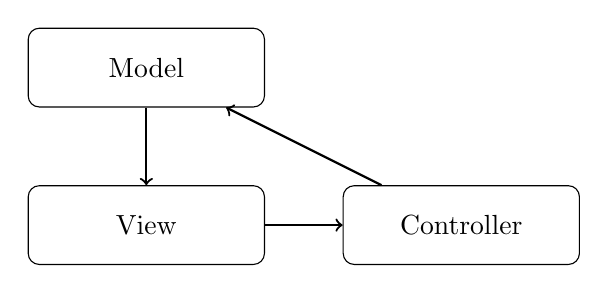
\begin{tikzpicture}[node distance=2cm]
\node (model) [rectangle, rounded corners, minimum width=3cm, minimum height=1cm, text centered, draw=black] {Model};
\node (view) [rectangle, rounded corners, minimum width=3cm, minimum height=1cm, text centered, draw=black, below of=model] {View};
\node (controller) [rectangle, rounded corners, minimum width=3cm, minimum height=1cm, text centered, draw=black, right of=view, xshift=2cm] {Controller};

\draw[->, thick] (controller) -- (model);
\draw[->, thick] (model) -- (view);
\draw[->, thick] (view) -- (controller);

\end{tikzpicture}
\caption{Схема архитектуры MVC}
\label{fig:mvc}
\end{figure}

MVC (Model-View-Controller) — одна из старейших и наиболее известных архитектурных парадигм. В этой архитектуре:

\begin{itemize}
    \item \textbf{Model} — представляет данные и бизнес-логику приложения. В контексте нашего туристического приложения это будут классы, представляющие туристические маршруты, достопримечательности, отзывы пользователей и другие бизнес-сущности.
    \item \textbf{View} — отвечает за отображение данных пользователю. В Flutter это будут виджеты, отображающие карты, списки маршрутов, профили пользователей.
    \item \textbf{Controller} — обрабатывает пользовательский ввод, взаимодействует с моделью и обновляет представление. Здесь будут находиться обработчики нажатий кнопок, логика фильтрации маршрутов и т.д.
\end{itemize}

\textbf{Плюсы MVC для нашего приложения:}
\begin{itemize}
    \item Простота внедрения и понимания — для небольшой команды разработчиков это упростит координацию.
    \item Хорошо подходит для простых экранов приложения, таких как страницы с описанием достопримечательностей или профили пользователей.
    \item Легко адаптировать существующие знания о MVC из других платформ.
\end{itemize}

\textbf{Минусы MVC для нашего приложения:}
\begin{itemize}
    \item Controller может стать «массивным» (так называемый "Massive View Controller"), особенно в экранах с большим количеством интерактивных элементов, например, при создании и редактировании маршрута.
    \item Тестируемость Controller затруднена из-за тесной связи с View.
    \item Масштабируемость ограничена — при добавлении новых функций (например, офлайн-режим для маршрутов) архитектура может стать запутанной.
\end{itemize}

\textbf{Применимость в приложении для путешествий:}
MVC может хорошо работать на начальных этапах разработки, но по мере добавления функциональности (например, интеграции геолокации, офлайн-режима, социальных функций для обмена маршрутами) структура может стать громоздкой. Для простых экранов, таких как просмотр информации о достопримечательностях, эта архитектура вполне подойдет, но для более сложных взаимодействий, таких как конструктор маршрутов, будут заметны ограничения.

\subsubsection*{MVP (Model-View-Presenter)}

\begin{figure}[H]
\centering
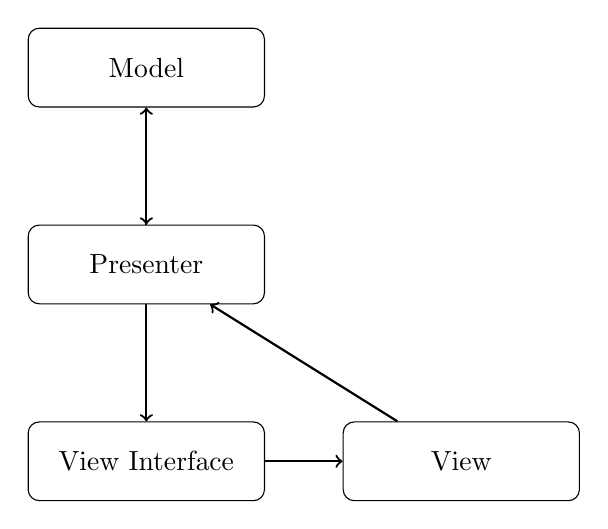
\begin{tikzpicture}[node distance=2.5cm]
% Верхний уровень
\node (model) [rectangle, rounded corners, minimum width=3cm, minimum height=1cm, text centered, draw=black] {Model};

% Средний уровень
\node (presenter) [rectangle, rounded corners, minimum width=3cm, minimum height=1cm, text centered, draw=black, below of=model] {Presenter};

% Нижний уровень
\node (vi) [rectangle, rounded corners, minimum width=3cm, minimum height=1cm, text centered, draw=black, below of=presenter] {View Interface};
\node (view) [rectangle, rounded corners, minimum width=3cm, minimum height=1cm, text centered, draw=black, right of=vi, xshift=1.5cm] {View};

\draw[->, thick] (presenter) -- (model);
\draw[->, thick] (model) -- (presenter);

\draw[->, thick] (presenter) -- (vi);
\draw[->, thick] (vi) -- (view);
\draw[->, thick] (view) -- (presenter);

\end{tikzpicture}
\caption{Схема архитектуры MVP}
\label{fig:mvp}
\end{figure}


MVP (Model-View-Presenter) — эволюция MVC, направленная на улучшение тестируемости и разделения ответственности:

\begin{itemize}
    \item \textbf{Model} — аналогично MVC, содержит данные и бизнес-логику. В нашем приложении это репозитории маршрутов, сервисы геолокации, хранилище избранных мест.
    \item \textbf{View} — пассивный элемент, который только отображает данные и передает пользовательские события в Presenter. Во Flutter это StatefulWidget или StatelessWidget с коллбэками.
    \item \textbf{Presenter} — содержит логику представления, реагирует на пользовательские действия, запрашивает данные от Model и обновляет View. Это будет класс, который обрабатывает действия, связанные с маршрутами, фильтрацией объектов и т.д.
\end{itemize}

\textbf{Плюсы MVP для нашего приложения:}
\begin{itemize}
    \item Лучшая тестируемость — Presenter не зависит от Flutter-виджетов, что делает его легко тестируемым с помощью unit-тестов.
    \item Чёткое разделение ответственности — облегчает разработку сложных экранов, таких как интерактивные карты маршрутов или поиск достопримечательностей.
    \item Улучшенная возможность повторного использования — Presenter может использоваться с разными реализациями View при необходимости (например, для разных размеров экрана).
\end{itemize}

\textbf{Минусы MVP для нашего приложения:}
\begin{itemize}
    \item Увеличение количества кода — требуется создание дополнительных интерфейсов между View и Presenter.
    \item Presenter всё ещё может становиться громоздким, особенно для сложных экранов с множеством функций (например, экран редактирования маршрута с добавлением фотографий, описаний, геолокаций).
    \item Двунаправленная зависимость между View и Presenter — не всегда идеальна для реактивных приложений.
\end{itemize}

\textbf{Применимость в приложении для путешествий:}
MVP обеспечивает лучшую структуру, чем MVC, для реализации сложных экранов приложения. Эта архитектура хорошо подойдет для экранов с активным взаимодействием, таких как создание маршрута, поиск и фильтрация мест. Разделение логики в Presenter позволит легко реализовать различные функции, связанные с планированием путешествий, и делать код более модульным. Однако для реактивных обновлений, например, при отслеживании текущей локации пользователя или отображении обновлений маршрута в реальном времени, могут потребоваться дополнительные паттерны.

\subsubsection*{MVVM (Model-View-ViewModel)}



\begin{figure}[H]
\centering
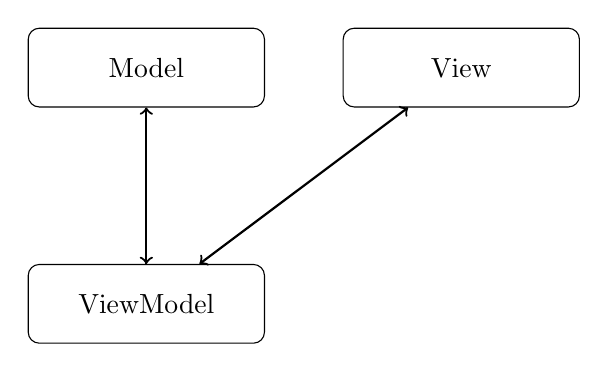
\begin{tikzpicture}[node distance=2.5cm]
\node (model) [rectangle, rounded corners, minimum width=3cm, minimum height=1cm, text centered, draw=black] {Model};
\node (view) [rectangle, rounded corners, minimum width=3cm, minimum height=1cm, text centered, draw=black, right of=model, xshift=1.5cm] {View};
\node (viewmodel) [rectangle, rounded corners, minimum width=3cm, minimum height=1cm, text centered, draw=black, below of=model, yshift=-0.5cm] {ViewModel};

\draw[->, thick] (viewmodel) -- (model);
\draw[->, thick, dashed] (model) -- (viewmodel);
\draw[<->, thick] (view) -- (viewmodel);

\end{tikzpicture}
\caption{Схема архитектуры MVVM}
\label{fig:mvvm}
\end{figure}


\subsubsection*{Применимость в приложении для путешествий}

В нашем приложении для внутреннего туризма:

\begin{itemize}
    \item \textbf{Model} включает классы для хранения информации о российских туристических местах, маршрутах, пользовательских данных.
    \item \textbf{View} представляет Flutter-виджеты для отображения списка маршрутов, карты достопримечательностей, экрана создания маршрута и т.д.
    \item \textbf{ViewModel} обрабатывает логику представления, такую как фильтрация маршрутов по регионам России, форматирование данных о достопримечательностях, обработка поиска и т.д.
\end{itemize}

\subsubsection*{Преимущества MVVM для нашего приложения}
\begin{itemize}
    \item \textbf{Двусторонняя привязка данных} — позволяет автоматически синхронизировать View и ViewModel, что удобно при создании интерактивных элементов для редактирования маршрутов.
    \item \textbf{Разделение обязанностей} — четкое разделение между UI и бизнес-логикой.
    \item \textbf{Хорошая тестируемость} — ViewModel можно тестировать независимо от View.
    \item \textbf{Переиспользуемость} — ViewModel не зависит от конкретного View, можно повторно использовать для разных представлений.
    \item \textbf{Управление состоянием} — хорошо подходит для сложных состояний приложения, например, для отслеживания прогресса создания маршрута пользователем.
\end{itemize}

\subsubsection*{Недостатки MVVM для нашего приложения}
\begin{itemize}
    \item \textbf{Сложность реализации для простых задач} — для простых экранов, таких как просмотр деталей достопримечательности, архитектура может быть избыточной.
    \item \textbf{Избыточное связывание} — для небольшого приложения может привести к излишней сложности.
    \item \textbf{Требует использования специальных инструментов} — для полноценной двухсторонней привязки во Flutter может потребоваться дополнительные библиотеки.
    \item \textbf{Кривая обучения} — освоение MVVM может занять больше времени для новых разработчиков проекта.
\end{itemize}

\subsubsection*{VIPER (View, Interactor, Presenter, Entity, Router)}

\subsubsection*{Описание архитектуры}

\begin{figure}[H]
\centering
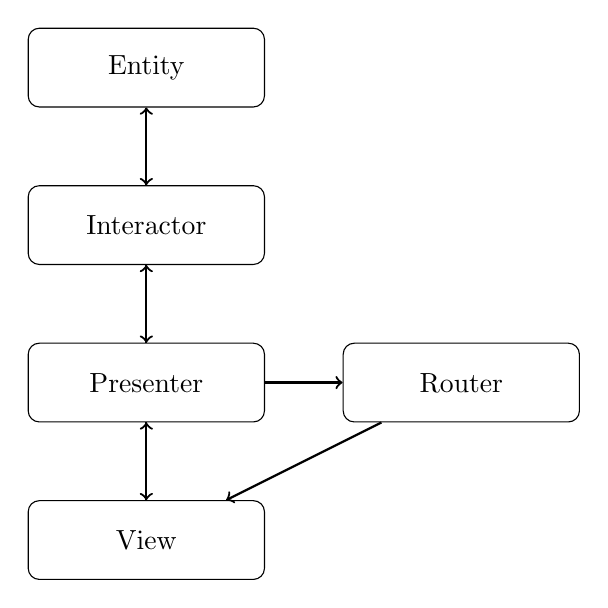
\begin{tikzpicture}[node distance=2cm]
% Верхний уровень - Entity
\node (entity) [rectangle, rounded corners, minimum width=3cm, minimum height=1cm, text centered, draw=black] {Entity};

% Средний уровень - Interactor и Presenter
\node (interactor) [rectangle, rounded corners, minimum width=3cm, minimum height=1cm, text centered, draw=black, below of=entity] {Interactor};
\node (presenter) [rectangle, rounded corners, minimum width=3cm, minimum height=1cm, text centered, draw=black, below of=interactor] {Presenter};

% Нижний уровень - View и Router
\node (view) [rectangle, rounded corners, minimum width=3cm, minimum height=1cm, text centered, draw=black, below of=presenter] {View};
\node (router) [rectangle, rounded corners, minimum width=3cm, minimum height=1cm, text centered, draw=black, right of=presenter, xshift=2cm] {Router};

% Связи
\draw[->, thick] (interactor) -- (entity);
\draw[->, thick] (entity) -- (interactor);

\draw[->, thick] (presenter) -- (interactor);
\draw[->, thick] (interactor) -- (presenter);

\draw[->, thick] (view) -- (presenter);
\draw[->, thick] (presenter) -- (view);

\draw[->, thick] (presenter) -- (router);
\draw[->, thick] (router) -- (view);

\end{tikzpicture}
\caption{Схема архитектуры VIPER}
\label{fig:viper}
\end{figure}





VIPER — архитектурный шаблон, который расширяет принцип разделения обязанностей до пяти компонентов:

\begin{itemize}
    \item \textbf{View} — отвечает за отображение данных и передачу действий пользователя Presenter.
    \item \textbf{Interactor} — содержит бизнес-логику, связанную с манипуляцией данными.
    \item \textbf{Presenter} — получает действия от View, запрашивает данные от Interactor и определяет, как эти данные будут представлены в View.
    \item \textbf{Entity} — модели данных, используемые Interactor.
    \item \textbf{Router} — отвечает за навигацию между модулями приложения.
\end{itemize}



\subsubsection*{Применимость в приложении для путешествий}

В контексте нашего приложения для внутреннего туризма:

\begin{itemize}
    \item \textbf{View} — Flutter-виджеты для отображения экранов приложения: списка маршрутов, карты регионов России, деталей достопримечательностей.
    \item \textbf{Interactor} — содержит логику для работы с данными туристических маршрутов, обработки пользовательских запросов, загрузки информации о местах.
    \item \textbf{Presenter} — форматирует данные для отображения и обрабатывает пользовательские действия (например, сохранение маршрута, добавление новой точки в маршрут).
    \item \textbf{Entity} — модели данных для маршрутов, мест, пользовательских профилей и т.д.
    \item \textbf{Router} — управляет навигацией между различными частями приложения (например, переход от списка маршрутов к детальному просмотру).
\end{itemize}

\subsubsection*{Преимущества VIPER для нашего приложения}
\begin{itemize}
    \item \textbf{Высокая модульность} — каждый модуль (экран) приложения является независимым, что упрощает разработку командой.
    \item \textbf{Отличная тестируемость} — компоненты разделены и могут тестироваться изолированно.
    \item \textbf{Четкое разделение обязанностей} — улучшает понимание кода и его поддержку.
    \item \textbf{Масштабируемость} — хорошо подходит для управления большими, сложными приложениями.
    \item \textbf{Структурированная навигация} — Router обеспечивает чистую организацию навигации между экранами, что важно для приложения с множеством маршрутов и мест.
\end{itemize}

\subsubsection*{Недостатки VIPER для нашего приложения}
\begin{itemize}
    \item \textbf{Избыточность для небольших приложений} — создает значительные накладные расходы для простых функций.
    \item \textbf{Большое количество классов} — может привести к фрагментации кода.
    \item \textbf{Высокая сложность} — сложно внедрять и поддерживать для небольшой команды.
    \item \textbf{Затраты на обучение} — требует значительного времени на обучение новых разработчиков.
    \item \textbf{Избыточность для Flutter} — некоторые концепции VIPER могут дублировать встроенные механизмы Flutter.
\end{itemize}

\subsubsection*{Model-View-Intent (MVI)}

\subsubsection*{Описание архитектуры}
\begin{figure}[H]
\centering
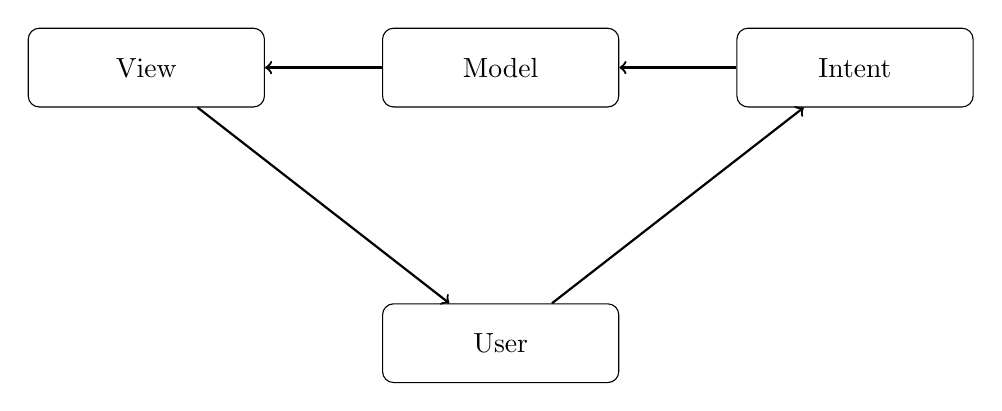
\begin{tikzpicture}[node distance=2.5cm]
% Верхний треугольник
\node (model) [rectangle, rounded corners, minimum width=3cm, minimum height=1cm, text centered, draw=black] {Model};
\node (view) [rectangle, rounded corners, minimum width=3cm, minimum height=1cm, text centered, draw=black, left of=model, xshift=-2cm] {View};
\node (intent) [rectangle, rounded corners, minimum width=3cm, minimum height=1cm, text centered, draw=black, right of=model, xshift=2cm] {Intent};

% User внизу
\node (user) [rectangle, rounded corners, minimum width=3cm, minimum height=1cm, text centered, draw=black, below of=model, yshift=-1cm] {User};

% Связи
\draw[->, thick] (user) -- (intent);
\draw[->, thick] (intent) -- (model);
\draw[->, thick] (model) -- (view);
\draw[->, thick] (view) -- (user);

\end{tikzpicture}
\caption{Схема архитектуры MVI}
\label{fig:mvi}
\end{figure}



MVI — однонаправленный и циклический архитектурный шаблон:

\begin{itemize}
    \item \textbf{Model} — представляет состояние приложения, является неизменяемым (immutable).
    \item \textbf{View} — отображает состояние и отправляет намерения пользователя.
    \item \textbf{Intent} — представляет намерение пользователя изменить состояние.
\end{itemize}

Основная концепция MVI — циклический поток данных: View генерирует Intent, Intent преобразуется в новое состояние Model, Model отображается View.



\subsubsection*{Применимость в приложении для путешествий}

В нашем приложении для внутреннего туризма:

\begin{itemize}
    \item \textbf{Model (State)} — представляет текущее состояние приложения, включая список маршрутов, выбранные фильтры, текущее местоположение пользователя.
    \item \textbf{View} — отображает текущее состояние (карту с маршрутами, список достопримечательностей) и отправляет намерения пользователя (создать новый маршрут, добавить место в избранное).
    \item \textbf{Intent} — представляет действия пользователя, такие как выбор региона России, создание маршрута, поиск достопримечательностей.
\end{itemize}

\subsubsection*{Преимущества MVI для нашего приложения}
\begin{itemize}
    \item \textbf{Предсказуемое управление состоянием} — особенно полезно для интерактивных функций приложения, таких как фильтрация маршрутов или создание новых маршрутов.
    \item \textbf{Отслеживаемость изменений} — каждое изменение состояния можно отследить, что полезно для отладки и журналирования.
    \item \textbf{Единое направление потока данных} — упрощает понимание того, как данные перемещаются в приложении.
    \item \textbf{Хорошая тестируемость} — поскольку состояние неизменяемо, тестирование становится более предсказуемым.
    \item \textbf{Устойчивость к параллельным операциям} — хорошо подходит для обработки асинхронных операций, таких как загрузка данных о туристических местах.
\end{itemize}

\subsubsection*{Недостатки MVI для нашего приложения}
\begin{itemize}
    \item \textbf{Излишнее создание объектов} — из-за неизменяемости состояния создается много новых объектов, что может влиять на производительность.
    \item \textbf{Сложность для простых случаев} — для простых экранов, таких как страница "О приложении", архитектура может быть избыточной.
    \item \textbf{Кривая обучения} — может быть сложно освоить для разработчиков, не знакомых с реактивным программированием.
    \item \textbf{Избыточное количество boilerplate-кода} — требуется написание большого количества шаблонного кода.
\end{itemize}

\subsubsection*{Business Logic Component (BLoC)}

\subsubsection*{Описание архитектуры}

\begin{figure}[H]
\centering
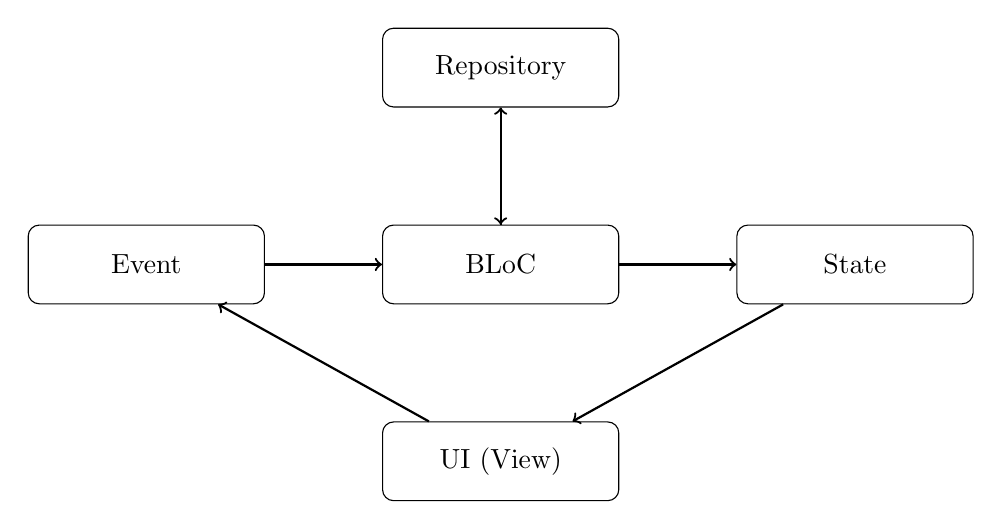
\begin{tikzpicture}[node distance=2.5cm]
% Компоненты BLoC
\node (repository) [rectangle, rounded corners, minimum width=3cm, minimum height=1cm, text centered, draw=black] {Repository};

\node (bloc) [rectangle, rounded corners, minimum width=3cm, minimum height=1cm, text centered, draw=black, below of=repository] {BLoC};

\node (event) [rectangle, rounded corners, minimum width=3cm, minimum height=1cm, text centered, draw=black, left of=bloc, xshift=-2cm] {Event};
\node (state) [rectangle, rounded corners, minimum width=3cm, minimum height=1cm, text centered, draw=black, right of=bloc, xshift=2cm] {State};

\node (ui) [rectangle, rounded corners, minimum width=3cm, minimum height=1cm, text centered, draw=black, below of=bloc] {UI (View)};

% Связи
\draw[->, thick] (bloc) -- (repository);
\draw[->, thick] (repository) -- (bloc);

\draw[->, thick] (event) -- (bloc);
\draw[->, thick] (bloc) -- (state);

\draw[->, thick] (ui) -- (event);
\draw[->, thick] (state) -- (ui);

\end{tikzpicture}
\caption{Схема архитектуры BLoC}
\label{fig:bloc}
\end{figure}


BLoC — архитектурный шаблон, специально разработанный для Flutter, основанный на реактивном программировании с использованием потоков (streams):

\begin{itemize}
    \item \textbf{BLoC (Business Logic Component)} — компонент, который принимает события от пользовательского интерфейса, обрабатывает их и выдает новое состояние через потоки.
    \item \textbf{Events (События)} — действия пользователя или системные события, которые инициируют изменения в приложении.
    \item \textbf{States (Состояния)} — различные состояния, которые может принимать приложение в ответ на события.
    \item \textbf{UI (Пользовательский интерфейс)} — реактивно обновляется в зависимости от состояния, полученного от BLoC.
\end{itemize}


\subsubsection*{Применимость в приложении для путешествий}

В нашем приложении для внутреннего туризма по России:

\begin{itemize}
    \item \textbf{BLoC} — обрабатывает бизнес-логику, такую как загрузка маршрутов, фильтрация по регионам России, поиск мест и создание новых маршрутов.
    \item \textbf{Events} — такие события, как "Загрузить маршруты", "Применить фильтр по региону", "Сохранить новый маршрут".
    \item \textbf{States} — состояния, такие как "Загрузка", "Данные загружены", "Ошибка загрузки", "Фильтр применен".
    \item \textbf{UI} — Flutter-виджеты, отображающие карту с маршрутами, список мест, экран создания маршрута.
\end{itemize}

\subsubsection*{Преимущества BLoC для нашего приложения}
\begin{itemize}
    \item \textbf{Идеально подходит для Flutter} — разработан специально для Flutter и хорошо интегрируется с его реактивным подходом.
    \item \textbf{Разделение UI и бизнес-логики} — UI становится декларативным и зависит только от состояния.
    \item \textbf{Простота тестирования} — бизнес-логика изолирована и может быть легко протестирована.
    \item \textbf{Реактивное программирование} — естественным образом поддерживает асинхронные операции, которые важны для туристического приложения (загрузка данных о местах, маршрутах).
    \item \textbf{Управление состоянием} — обеспечивает централизованное и предсказуемое управление состоянием.
    \item \textbf{Большое сообщество и поддержка} — многочисленные библиотеки и документация.
    \item \textbf{Масштабируемость} — хорошо работает как с небольшими, так и с крупными приложениями.
\end{itemize}

\subsubsection*{Недостатки BLoC для нашего приложения}
\begin{itemize}
    \item \textbf{Избыточный код для простых случаев} — для простых экранов, таких как информационные страницы о региональных особенностях, может быть избыточным.
    \item \textbf{Кривая обучения} — новичкам во Flutter может потребоваться время для освоения концепций потоков и реактивного программирования.
    \item \textbf{Сложность отладки} — асинхронный характер потоков может усложнить отладку.
    \item \textbf{Поддержка состояния} — для очень сложных состояний может потребоваться дополнительная работа.
\end{itemize}


Таким образом, для управления состоянием нами был выбран паттерн \textbf{BLoC} (Business Logic Component). BLoC помогает отделить бизнес-логику от UI, делая код более структурированным, тестируемым и предсказуемым. Подробное описание архитектуры BLoC (события, состояния, потоки) было приведено в исходной версии данной главы.

Ключевые преимущества BLoC для данного проекта:
\begin{itemize}
    \item \textbf{Реактивность}: Идеально подходит для Flutter, позволяя UI декларативно реагировать на изменения состояния.
    \item \textbf{Разделение ответственности}: Четкое разделение UI от бизнес-логики. UI отправляет события в BLoC и слушает поток состояний.
    \item \textbf{Тестируемость}: BLoC можно легко тестировать изолированно, проверяя преобразование событий в состояния.
    \item \textbf{Масштабируемость}: Подходит для управления как простыми, так и сложными состояниями.
\end{itemize}
Библиотека \textit{flutter\_bloc} предоставляет удобные инструменты для реализации этого паттерна.



\subsection*{Ключевые архитектурные принципы и подходы}

Кроме того, при всем процессе разработки важно придерживаться общепризнанных принципов проектирования программного обеспечения, таких как SOLID, KISS, DRY, и концепциях объектно-ориентированного программирования.  


\subsubsection*{Ключевые архитектурные принципы}
\textbf{Принципы SOLID}.
Акроним SOLID обозначает пять основных принципов объектно-ориентированного проектирования, предложенных Робертом Мартином:
\begin{itemize}
    \item \textbf{S – Принцип единственной ответственности (Single Responsibility Principle – SRP)}: Каждый класс или модуль должен иметь одну и только одну причину для изменения. В контексте приложения это означает, например, что BLoC отвечает за управление состоянием конкретного экрана или фичи, репозиторий – за доступ к данным определенного типа, а виджет – за отображение части пользовательского интерфейса.
    \item \textbf{O – Принцип открытости/закрытости (Open/Closed Principle – OCP)}: Программные сущности (классы, модули, функции) должны быть открыты для расширения, но закрыты для модификации. Это достигается за счет использования абстракций и полиморфизма, позволяя добавлять новую функциональность без изменения существующего рабочего кода.
    \item \textbf{L – Принцип подстановки Барбары Лисков (Liskov Substitution Principle – LSP)}: Объекты в программе должны быть заменяемы экземплярами их подтипов без изменения правильности выполнения программы. Это важно при работе с наследованием и интерфейсами, гарантируя, что производные классы могут использоваться там, где ожидаются базовые.
    \item \textbf{I – Принцип разделения интерфейса (Interface Segregation Principle – ISP)}: Клиенты не должны быть вынуждены зависеть от интерфейсов, которые они не используют. Предпочтительнее создавать небольшие, специфичные интерфейсы, чем один большой универсальный. Это актуально при определении контрактов для репозиториев или сервисов.
    \item \textbf{D – Принцип инверсии зависимостей (Dependency Inversion Principle – DIP)}: Модули верхних уровней не должны зависеть от модулей нижних уровней. И те, и другие должны зависеть от абстракций. Абстракции не должны зависеть от деталей. Детали должны зависеть от абстракций. Этот принцип является ключевым для построения слабосвязанных систем. В приложении он реализуется через использование интерфейсов (абстракций) для репозиториев, которые внедряются в BLoC или другие бизнес-компоненты.
\end{itemize}

\textbf{KISS (Keep It Simple, Stupid)}.
Этот принцип призывает к простоте дизайна и реализации. Следует избегать излишней сложности и выбирать наиболее прямолинейное решение, которое удовлетворяет требованиям. Простой код легче понимать, тестировать и поддерживать.

\textbf{DRY (Don't Repeat Yourself)}.
Принцип "Не повторяйся" нацелен на избежание дублирования кода. Повторяющиеся участки кода следует выносить в отдельные функции, классы или компоненты, чтобы обеспечить их многократное использование. Это повышает поддерживаемость и снижает вероятность ошибок при внесении изменений.

\textbf{Многоуровневое разделение ответственности (Layering)}.
Приложение структурировано с использованием многоуровневого подхода, где каждый слой имеет четко определенную зону ответственности. Это способствует лучшей организации кода, повышает его тестируемость и позволяет независимую разработку и модификацию отдельных частей системы. Основные логические слои включают:
\begin{itemize}
    \item \textbf{Слой представления (Presentation Layer)}: Отвечает за отображение информации пользователю и обработку его ввода. Включает виджеты Flutter и компоненты управления состоянием (BLoC), которые адаптируют данные для отображения и передают действия пользователя в нижележащие слои.
    \item \textbf{Слой бизнес-логики (Business Logic/Domain Layer)}: Содержит основные бизнес-правила, сущности предметной области (модели данных) и логику их взаимодействия. Этот слой не зависит от деталей UI или источников данных. Включает модели (например, \textit{RouteModel}, \textit{PlaceModel}) и, при необходимости, сервисы или интеракторы, инкапсулирующие сложные операции.
    \item \textbf{Слой доступа к данным (Data Layer)}: Обеспечивает взаимодействие с источниками данных, такими как удаленный сервер (через gRPC) или локальное хранилище. Включает реализации репозиториев, которые абстрагируют детали получения и сохранения данных от слоя бизнес-логики.
\end{itemize}

\textbf{Правило зависимостей (Dependency Rule)}.
Важным аспектом многоуровневой архитектуры является направление зависимостей. Зависимости должны быть направлены "внутрь" – от слоев, отвечающих за внешние детали (UI, база данных), к слоям, содержащим основную бизнес-логику. Слой бизнес-логики не должен знать о конкретных реализациях UI или источников данных. Это достигается за счет использования абстракций (интерфейсов) и принципа инверсии зависимостей (DIP). Например, слой бизнес-логики (или BLoC в слое представления) зависит от интерфейса репозитория, а не от его конкретной реализации, которая предоставляется через механизм внедрения зависимостей.

Эта комбинация принципов и подходов позволяет создать гибкую, масштабируемую и поддерживаемую архитектуру для мобильного приложения "Путешествия по России".


Применение Чистой архитектуры способствует независимости от фреймворков, тестируемости бизнес-логики без UI и базы данных, а также лучшей организации кода.

\subsubsection*{Подход "Feature-First" к организации кода}
Для структурирования проекта был выбран подход \textbf{Feature-First}. Это означает, что код группируется не по техническим слоям (например, все виджеты в одной папке, все модели в другой), а по функциональным модулям (фичам). Каждая фича (например, "просмотр списка маршрутов", "создание маршрута") инкапсулирует все необходимые для ее работы компоненты: UI, управление состоянием (BLoC), бизнес-логику (если она специфична для фичи и не вынесена в общие Use Cases), и модели данных.

Такой подход улучшает локализацию изменений: при модификации фичи изменения, как правило, затрагивают только ее папку. Это также облегчает навигацию по проекту и параллельную работу нескольких разработчиков над разными фичами. Внутри каждой фичи код может быть дополнительно структурирован по слоям (например, \textit{ui}, \textit{bloc}, \textit{domain}, \textit{data}).



\subsubsection*{Внедрение зависимостей (DI) с yx\_scope}
Для управления зависимостями (Dependency Injection, DI) в проекте был выбран фреймворк \textbf{yx\_scope}. Разработанный в Яндексе, \textbf{yx\_scope} представляет собой DI-фреймворк, нацеленный на упорядочивание работы со скоупами \footnote{Скоуп (scope) в контексте yx\_scope – это контейнер с набором зависимостей, который существует только определённое время. Создание и удаление отдельного скоупа происходит по заранее описанным условиям в процессе работы приложения. В приложении может существовать несколько скоупов с разными жизненными циклами.}. в больших и многомодульных проектах.

Ключевая задача, которую решает \textbf{yx\_scope} – унификация подхода к управлению зависимостями в условиях, когда разные команды или модули могут использовать различные DI-решения (например, getIt, injectable, Riverpod), что усложняет взаимодействие и поддержку проекта. \textbf{yx\_scope} был создан с целью удовлетворить следующий набор требований: чистый Dart \footnote{Dart – язык программирования, созданный Google, оптимизированный для клиентской разработки веб- и мобильных приложений. Является основным языком для фреймворка Flutter.}, DI-подобный подход (не статика и не ServiceLocator), отсутствие кодогенерации для основной функциональности, возможность встраивания DI-контейнера в виджеты \footnote{Виджет (Widget) в Flutter – основной строительный блок пользовательского интерфейса. Все, что отображается на экране, является виджетом, от простого текста до сложных компоновок.}, нереактивное и декларативное дерево зависимостей, однозначное поведение и жизненный цикл зависимостей, поддержка вложенных скоупов любой глубины, асинхронные зависимости и их инициализация, а также compile-safe \footnote{Compile-safe (безопасность на этапе компиляции) – свойство системы типов или инструмента разработки, которое позволяет обнаруживать определённые классы ошибок во время компиляции программы, а не в рантайме.} доступ к зависимостям и защита от циклических зависимостей.

Фреймворк состоит из трёх основных библиотек:
\begin{itemize}
    \item yx\_scope: ядро реализации, основной «движок».
    \item yx\_scope\_flutter: библиотека-адаптер, позволяющая интегрировать контейнеры \textbf{yx\_scope} в дерево виджетов Flutter \footnote{Flutter – это UI SDK (набор инструментов разработки пользовательского интерфейса) с открытым исходным кодом, созданный Google. Используется для создания нативных кроссплатформенных приложений из единой кодовой базы для мобильных устройств (iOS, Android), веба и десктопа.}.
    \item yx\_scope\_linter: набор кастомных правил статического анализа (lint-правил) для дополнительной защиты от ошибок при работе с фреймворком.
\end{itemize}

Ключевые особенности и преимущества \textbf{yx\_scope}:
\begin{itemize}
    \item \textbf{Безопасность на этапе компиляции (Compile-safety)}: Гарантирует, что если код компилируется, он будет корректно работать в части DI.
    \item \textbf{Простота}: В базовых сценариях синтаксис и поведение схожи с другими известными DI-решениями.
    \item \textbf{Масштабируемость}: Скоупы легко создаются, связываются и изменяются, позволяя скрывать сложность DI за абстракциями.
    \item \textbf{Чистый Dart, но Flutter-friendly}: DI-контейнер не зависит от UI, но легко интегрируется с Flutter, используя привычные паттерны.
\end{itemize}

Основные понятия в \textbf{yx\_scope}:
\begin{itemize}
    \item \textbf{Dep (зависимость)}: Контейнер для одного конкретного экземпляра зависимости.
    \item \textbf{Scope (скоуп)}: Контейнер, который определяет, какие зависимости (Deps) будут в нём созданы и как они будут связаны друг с другом. Это декларативное описание набора зависимостей.
    \item \textbf{ScopeHolder}: Сущность, которая «держит» активный экземпляр Scope. ScopeHolder отвечает за создание, существование и удаление инстанса скоупа. Важно, что ScopeHolder не является статическим, что обеспечивает локализацию скоупов.
    \item \textbf{ScopeProvider} и \textbf{ScopeBuilder}: Виджеты из библиотеки \texttt{yx\_scope\_flutter}, предназначенные для интеграции скоупов в дерево виджетов Flutter, обеспечивая доступ к зависимостям из UI.
\end{itemize}

В данном приложении \textbf{yx\_scope} используется для определения нескольких уровней скоупов: глобальный \textit{AppScope} для общеприложенческих зависимостей (например, gRPC \footnote{gRPC (gRPC Remote Procedure Calls) – это современный высокопроизводительный фреймворк RPC (удаленного вызова процедур) с открытым исходным кодом, который может работать в любой среде.} клиент, главный репозиторий \footnote{Репозиторий (Repository) – паттерн проектирования, который разделяет логику доступа к данным от бизнес-логики, предоставляя интерфейс для работы с сущностями как с коллекцией объектов.}, сервис логирования), \textit{ContentScope} для фич, связанных с отображением основного контента, и более локальные скоупы, такие как \textit{CreateRouteScope} для фичи создания маршрута. Эта иерархия позволяет эффективно управлять жизненным циклом зависимостей, соотнося его с жизненным циклом фич, что хорошо согласуется с Feature-First подходом к организации проекта.



\subsubsection*{Взаимодействие с бэкендом: gRPC}
Для сетевого взаимодействия между мобильным приложением и серверной частью был выбран протокол \textbf{gRPC}. gRPC (Google Remote Procedure Call) — это современный, высокопроизводительный фреймворк RPC с открытым исходным кодом, который может работать в любой среде.

Ключевые причины выбора gRPC:
\begin{itemize}
    \item \textbf{Производительность}: gRPC использует HTTP/2 для передачи данных и Protocol Buffers (Protobuf) в качестве языка описания интерфейсов и формата сериализации сообщений. Protobuf обеспечивает эффективную бинарную сериализацию, что приводит к меньшему объему передаваемых данных и более низкой задержке по сравнению с текстовыми форматами, такими как JSON, используемыми в REST API.
    \item \textbf{Строгая типизация и контракты}: Описание сервисов и сообщений с помощью \textit{.proto} файлов обеспечивает строгую типизацию данных и четкие контракты между клиентом и сервером. Это снижает вероятность ошибок интеграции и упрощает эволюцию API.
    \item \textbf{Кодогенерация}: Инструменты gRPC автоматически генерируют клиентский и серверный код на различных языках (включая Dart для Flutter) на основе \textit{.proto} файлов. Это избавляет от необходимости писать boilerplate-код для сетевых вызовов и парсинга данных.
    \item \textbf{Потоковая передача (Streaming)}: gRPC нативно поддерживает различные типы потоковой передачи данных (серверный, клиентский, двунаправленный), что может быть полезно для реализации интерактивных функций и передачи больших объемов данных.
\end{itemize}
Контракты взаимодействия с бэкендом описываются в \textit{.proto} файлах, размещенных в директории \textit{lib/src/proto/}. На их основе генерируется Dart-код для gRPC клиента, который используется в слое данных приложения.





